\section{Ionic Liquid Gating Technique}
\label{sec:expsetup:ionicliquid}

Ionic liquid gating technique is a novel gating approach. Similar to the traditional solid gating method, ionic liquid gating also leverages a thin capacitor to change the chemical potential on the surface of a sample. One plate of the capacitance is also the sample surface. But unlike the solid state gating, the other capacitance plate is one layer of ions in the ionic liquid. Besides, since the ions sit on top of the sample surface, the thickness of the capacitor is on the order of the atomic scale. Thus it provides a very large capacitance and leads to a powerful gating effect. Previously, Iwasa's group first demonstrated the power of ionic liquid on ZnO\cite{yuan2009ZnO}. Then together with Iwasa\cite{Yuan2011}, Ando \cite{Ando_liquid} and Tokura group\cite{Checkelsky_liquid}, we introduced this novel gating method into TI transport experiments\cite{Xiong2013}. We discuss some technical details of the ionic liquid gating experiments here. 

The ionic liquid we use is DEME-TFSI, comprised of cations (CH$_3$ CH$_2$ )$_2$ (CH$_2$ CH$_2$ OCH$_3$ )CH$_3$ N$^+$ and anions (CF$_3$SO$_2$)$_2$N$_-$. This ionic liquid has been proved to provide a powerful gating effect in previous experiments\cite{yuan2009ZnO, ye2010liquid}. Before using the liquid, we pump it at $25 \,^{\circ}{\rm C}$ for 2 hours in order to minimize any water content that can accelerate unfavorable chemical reactions. Then the sample, the ionic liquid and the gold gate plate are put into a sapphire container (as shown in Fig. \ref{ILcontain}), and are quickly loaded into the cryostat. Then the sample is fast cooled down to around 220 K to diminish any chemical reaction or damage that may happen to the sample before the liquid freezes. As displayed by Fig. \ref{ILcontain}, there is a gold plate at the bottom of the container that serves as the gate electrode. Above the ionic liquid melting temperature, when a gate voltage is applied between the sample and the gold plate, ions will move inside the liquid. If the gate voltage $V_G$ is positive, cations will drift away from the gate plate and come to the sample surface, while anions will leave the sample. As a result, there forms a thin layer of extra cations on the sample surface, and these ions will generate a strong electric field towards the sample and lift its chemical potential. 

Starting from 0 V, we then apply a gate voltage $V_G$ to the gold plate at a �gating temperature� around 220 K at a sweeping speed of approximately 1 V/min. After the planned $V_G$ is attained, the sample is quickly cooled to 160 K to reduce the possibility of chemical reactions. Then the sample and the liquid are cooled down to 4 K slowly (at 2 K/min) to reduce the stress on the sample and the contacts caused by the freezing ionic liquid. The cooling process has a possibility to damage the sample as we find that repeated freezing and thawing of the ionic liquid can snap the leads or the crystal itself. At 4 K, the large $E$-field induced by the frozen surface anion density $N_{ion}$ (1-4$\times 10^{14}$ cm$^{-2}$) creates a depletion layer that changes the chemical potential in the sample significantly.

Unfortunately, the large gating power is not free. It is more difficult to change the gating voltage with the ionic liquid than using the solid-state gating. Every time we change $V_G$, we need to slowly (at 2 K/min) warm up the sample to the "gating temperature" around 220 K and change $V_G$ by small steps. At the "gating temperature", a typical way to change $V_G$ is to change it in steps of $\sim$0.02 V every 5 to 10 seconds, while monitoring the transient current $I_{trans}$ (1-40 nA). The time spent at the "gating temperature" is typically 300-500 s. Then the sample is cooled down to 5 K with the gating voltage fixed as we discussed above. To minimize the sample damage, we start at $V_G$ = 0 V during the first cool-down, followed by measurements at increasingly negative $V_G$ until the sample fails (usually by a discharge event).  We emphasize that the changes to the resistivity $\rho$ and the Hall density $n_H$ are reversible (see below) as long as $|V_G|$ does not exceed a limit. Upon returning $V_G$ to 0 V, we could recover the same starting value of R (at 5 K) provided $|V_G|$  is kept below 2 V.

\begin{figure}[!htbp]
  \begin{center}
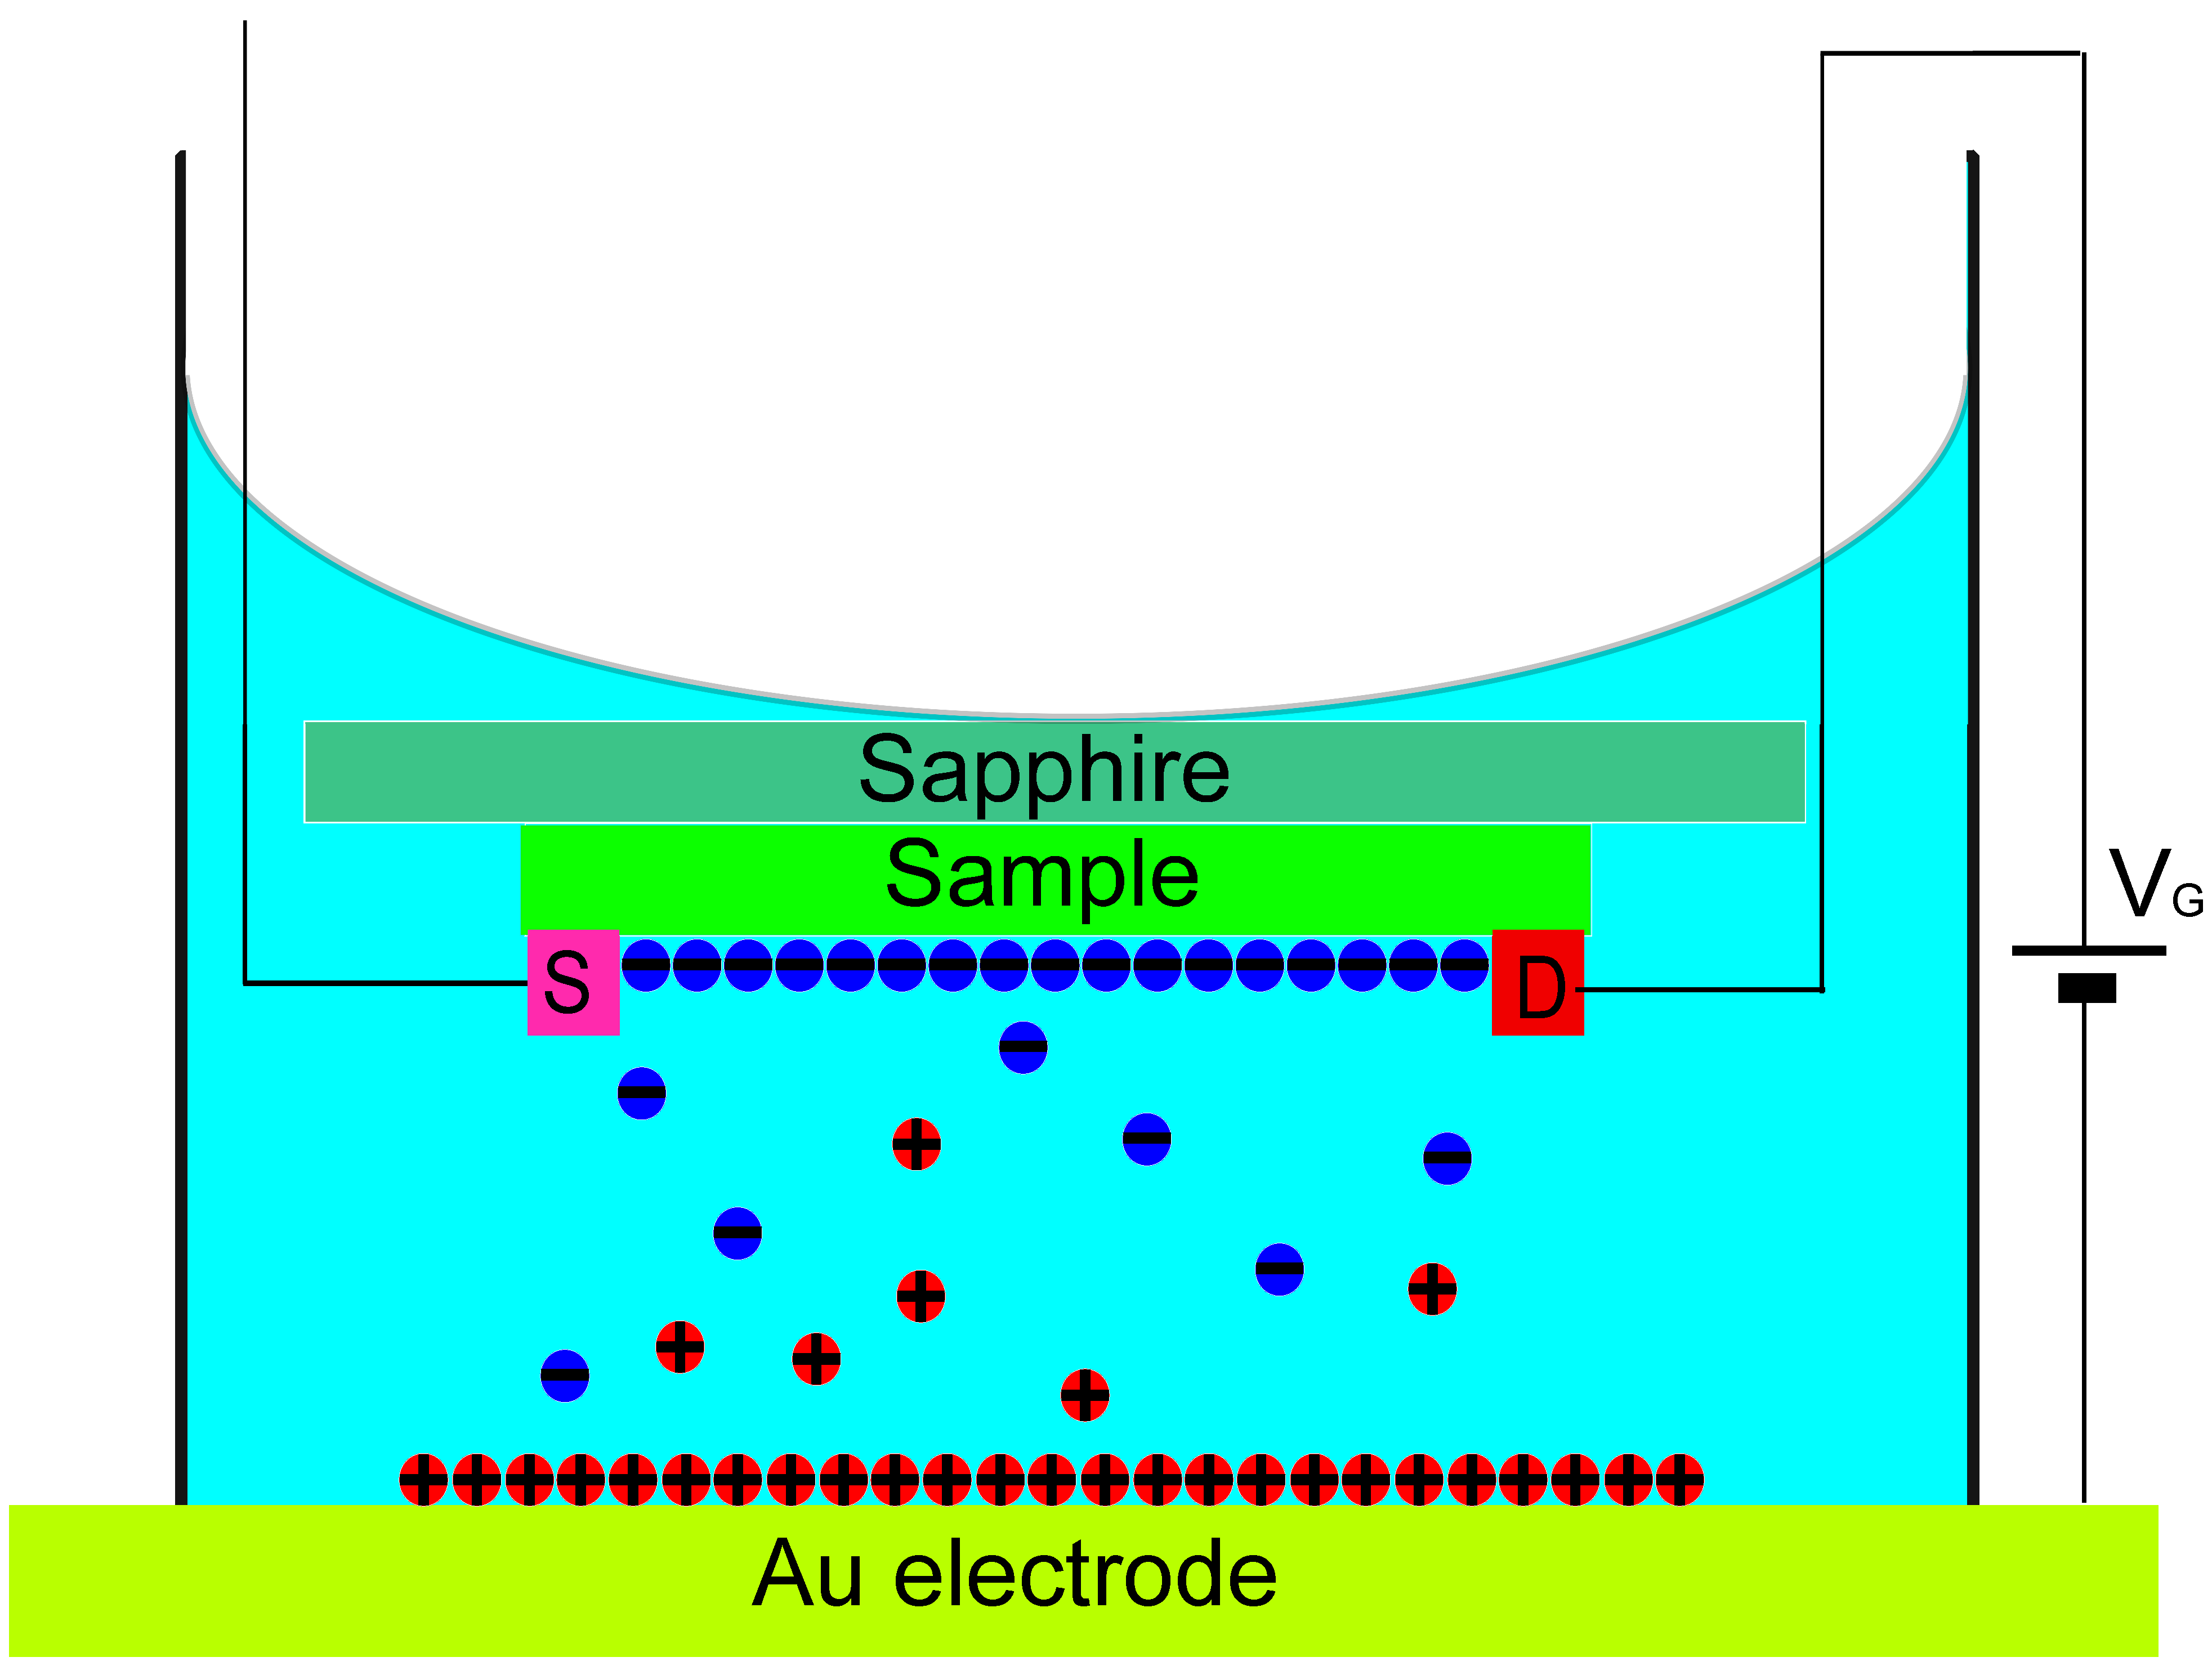
\includegraphics[width=0.8\linewidth]{ch-expsetup/figures/ILcontain.eps}
\caption{\label{ILcontain}
The configuration of the ionic liquid gating experiment. Both the ionic liquid and the sample are held in a sapphire container with a gold plate at the bottom. The Au plate is used to apply a gating voltage to the sample.}
  \end{center}
\end{figure}